\documentclass[conference,final]{IEEEtran}

\usepackage{latex8}
\usepackage{times}

\usepackage[utf8]{inputenc}
\usepackage{url}
\usepackage{float}
\usepackage{times}    
\usepackage{multirow}    
\usepackage{listings}   
\usepackage{times}     
\usepackage{paralist}    
\usepackage{wrapfig}    
\usepackage[small,it]{caption}
\usepackage{multirow}
\usepackage{ifpdf}
%\usepackage{srcltx}
\usepackage{subfigure}
\usepackage{paralist}

\usepackage{listings}
\usepackage{keyval}  
\usepackage{color}
\definecolor{listinggray}{gray}{0.95}
\definecolor{darkgray}{gray}{0.7}
\definecolor{commentgreen}{rgb}{0, 0.4, 0}
\definecolor{darkblue}{rgb}{0, 0, 0.4}
\definecolor{middleblue}{rgb}{0, 0, 0.7}
\definecolor{darkred}{rgb}{0.4, 0, 0}
\definecolor{brown}{rgb}{0.5, 0.5, 0}

\usepackage[normalem]{ulem}
\makeatletter
\def\cyanuwave{\bgroup \markoverwith{\lower3.5\p@\hbox{\sixly \textcolor{cyan}{\char58}}}\ULon}
\def\reduwave{\bgroup \markoverwith{\lower3.5\p@\hbox{\sixly \textcolor{red}{\char58}}}\ULon}
\def\blueuwave{\bgroup \markoverwith{\lower3.5\p@\hbox{\sixly \textcolor{blue}{\char58}}}\ULon}
\font\sixly=lasy6 % does not re-load if already loaded, so no memory problem.
\makeatother

\newif\ifdraft
\drafttrue
\ifdraft
\newcommand{\onote}[1]{ {\textcolor{cyan} { (***Ole: #1) }}}
\newcommand{\terminology}[1]{ {\textcolor{red} {(Terminology used: \textbf{#1}) }}}
\newcommand{\owave}[1]{ {\cyanuwave{#1}}}
\newcommand{\jwave}[1]{ {\reduwave{#1}}}
\newcommand{\alwave}[1]{ {\blueuwave{#1}}}
\newcommand{\jhanote}[1]{ {\textcolor{red} { ***shantenu: #1 }}}
\newcommand{\alnote}[1]{ {\textcolor{blue} { ***andre: #1 }}}
\newcommand{\amnote}[1]{ {\textcolor{blue} { ***andre2: #1 }}}
\newcommand{\smnote}[1]{ {\textcolor{green} { ***sharath: #1 }}}
\newcommand{\msnote}[1]{ {\textcolor{cyan} { ***mark: #1 }}}
\newcommand{\note}[1]{ {\textcolor{magenta} { ***Note: #1 }}}
\else
\newcommand{\onote}[1]{}
\newcommand{\terminology}[1]{}
\newcommand{\owave}[1]{#1}
\newcommand{\jwave}[1]{#1}
\newcommand{\alnote}[1]{}
\newcommand{\amnote}[1]{}
\newcommand{\athotanote}[1]{}
\newcommand{\smnote}[1]{}
\newcommand{\jhanote}[1]{}
\newcommand{\msnote}[1]{}
\newcommand{\note}[1]{}
\fi

\lstdefinestyle{myListing}{
  frame=single,   
  backgroundcolor=\color{listinggray},  
  %float=t,
  language=C,       
  basicstyle=\ttfamily \footnotesize,
  breakautoindent=true,
  breaklines=true
  tabsize=2,
  captionpos=b,  
  aboveskip=0em,
  belowskip=-2em,
  %numbers=left, 
  %numberstyle=\tiny
}      

\lstdefinestyle{myPythonListing}{
  frame=single,   
  backgroundcolor=\color{listinggray},  
  %float=t,
  language=Python,       
  basicstyle=\ttfamily \footnotesize,
  breakautoindent=true,
  breaklines=true
  tabsize=2,
  captionpos=b,  
  %numbers=left, 
  %numberstyle=\tiny
}

\newcommand{\up}{\vspace*{-1em}}
\newcommand{\upp}{\vspace*{-0.5em}}
\newcommand{\numrep}{8 }
\newcommand{\samplenum}{4 }
\newcommand{\tmax}{$T_{max}$ }
\newcommand{\tc}{$T_{C}$ }
\newcommand{\tcnsp}{$T_{C}$}
\newcommand{\bj}{BigJob}

% This is now the recommended way for checking for PDFLaTeX:
\usepackage{ifpdf}

%\newif\ifpdf
%\ifx\pdfoutput\undefined
%\pdffalse % we are not running PDFLaTeX
%\else
%\pdfoutput=1 % we are running PDFLaTeX
%\pdftrue
%\fi

\ifpdf
\usepackage[pdftex]{graphicx}
\else
\usepackage{graphicx}
\fi

% \title{Towards A Framework for Pilot-Abstractions for Production
%   Cyberinfrastructure}

%\title{P*: An Extensible Model of Pilot-Abstractions for Dynamic Execution}

\title{P*: An Extensible Model of Pilot-Abstractions}

% \jhanote{Alternate title: The Tiered Resource OverlaY framework
%   (TROY): An Empirical Framework for Pilot-* Abstractions}
% 
% \jhanote{old title: TROY -- Tiered Resource Overlay Framework: Towards
%   a Framework for Pilot-Abstractions for Distributed
%   Cyberinfrastructure}


\date{}

\begin{document}

\ifpdf
\DeclareGraphicsExtensions{.pdf, .jpg, .tif}
\else
\DeclareGraphicsExtensions{.eps, .jpg}
\fi

\author{
  Andre Luckow$^{1}$, Mark Santcroos$^{2,1}$, Sharath Maddineni$^{1}$, Andre Merzky$^{1}$, Ole Weidner$^{1}$, Shantenu Jha$^{3,1*}$\\
  \small{\emph{$^{1}$Center for Computation \& Technology, Louisiana State University, USA}}\\
 \small{\emph{$^{2}$Bioinformatics Laboratory, Academic Medical Center, University of Amsterdam, The Netherlands}}\\
 \small{\emph{$^{3}$ Rutgers University, Piscataway, NJ 08854, USA}}\\
  \small{\emph{$^{*}$Contact Author: \texttt{shantenu.jha@rutgers.edu}}}\\
  \up\up\up\up }

\maketitle

\begin{abstract}
  \up Distributed cyberinfrastructures (CI) and applications require
  the ability to determine and utilize resource selection at runtime
  (dynamically), and not just before execution (statically).
  Pilot-Jobs have been notable in their ability to support dynamic
  resource utilization -- in the number of applications that use them,
  in the scope of usage, as well as the number of CI that support
  them.  In spite of broad uptake, there does not exist however, a
  well defined, unifying conceptual framework for pilot-jobs which can
  be used to define, compare and contrast different
  implementations. This presents a barrier to extensibility and
  interoperability. This paper is an attempt to (i) provide a minimal
  but complete model (P*) of pilot-jobs, (ii) extend the basic model
  (but not implementation) from compute to data, (iii) introduce TROY
  as an implementation of this model, % using SAGA, i.\,e.\ consistent
%   with its API, job-model etc.,
  (iv) establish the generality of the P* model by mapping various
  existing and well known pilot-job frameworks such as CONDOR and
  DIANE to P*, (v) establish and validate the implementation of TROY
  by concurrently using multiple {\it distinct} pilot-jobs. \upp\upp\upp\upp
\end{abstract}

%\note{
% \section*{Outline}
% The primary objectives of this work are:
% \begin{enumerate}
% \item Establish the need for dynamic execution of applications -
%   distributed as well as high-end performance.
% \item We define the basic characteristics of the dynamic apps and we
%   understand the requirements of dynamic apps need to do in a
%   distributed environment.
% \item We understand the capability that must be provided by the
%   infrastructure to support these application
% \item We describe the pilot-job as a good prototype of an abstraction
%   that supports dynamic execution
% \item We define the characteristics that need to be supported by a
%   pilot-job \jhanote{Infrastructure or Application characteristics?}
%   \alnote{I think we meant application characteristics}
% \item There exist multiple PJ implementations out there but no way to
%   compare and contrast. Provide a framework to aid an understanding of
%   pilot-jobs and the ability to compare, contrast and understand
%   different pilot-jobs.  Provide both a theoretical and empirically
%   useful approach to determining which PJ to use
% \item Empirical implementation of TROY and demonstration of
%   concurrent/interoperation between equivalent but distinct Pilot-Job
%   implementation. Highlight unique feature of Troy: User extensible
%   and customizable. \jhanote{We should talk about this in light of the
%     reviews of the paper with Bishop}
% \end{enumerate}
%   Points 1-3 can go into the beginning of \S2.  Points 4 \& 5 should
%   be addressed in both introduction (see one of the \jhanote{} above),
%   as well as in the beginning of \S2. Points 6, 7 are addressed in the
%   Introduction.  }

%execution model, effectively equivalent to
%The two approaches can be viewed as different approaches to the
%dynamic resource problem.
%in one, the supply is kept fixed and the demand is changed to meet the
%supply; in the other the supply changes in response to the demand.

%For the purposes of this paper, we will focus on the latter, wherein
%the availability and utilization of resources changes.  As a
%consequence, we will not consider dynamic execution arising from
%internal application changes.  
%In other words, 


% Typically, this will involve a single ``large'' distributed
% application, that is comprised of many smaller tasks.\alnote{it
%   would be good if we could relate to our DARE use case here}

% \alnote{not sure why do we need week and strong model? Determinism and
%   distributed systems don't go together well. Also, I wouldn't claim
%   that the prob. of adv. rerv. is 1 (it might be 0.99...). PJ are more
% d  in line with the weak model. Do we say that Advance Reserv. are
%   better?}  \jhanote{Addressed.} \jhanote{OK to remove?}

% There exist two models of dynamic resource utilization, which we refer
% to as the weak (probabilistic) model of dynamic execution (DE) and the
% strong (deterministic) model of DE. In the former, there exists a
% certain probability to acquire a resource at a given instant of time;
% in the latter the probability of acquiring a resource is by definition
% is 1, but there exists a broad range of times over which this
% probability will first be 1. 

%or utilization ability.  this has the resultant effect of an
%application being dynamic, though dynamic resource execution maybe
%just one of multiple responses.

\section{Introduction and Overview \upp\upp}

\alnote{We use the term agent to denote a component inside the pilot
  that has some decision making capability. In most cases we could
  replace agent just with pilot. However, when talking about decentral
  coordination with autonomic decision making this will be
  difficult. Should we explicitly define an agent in sec II under
  Pilot-Job (aka pilot)?}
 
Distributed CI almost by definition is comprised of a set of resources
that is fluctuating -- growing, shrinking, changing in load and
capability.  The ability to utilize such a dynamic resource pool is
thus an important attribute of any application that needs to utilize
distributed CI efficiently; this is in contrast to a static resource
utilization model characteristic of parallel and cluster computing.

In addition, the evolution or internal dynamics of an application may
vary, thereby changing the resource requirements.
For example, different solvers, % or granularity of existing solvers,
adaptive algorithms and/or implementations, can also require
applications to utilize different set/amounts of resources.
%provide applications with a dynamic resource utilization requirements.  
We will define dynamic applications to have the ability to respond to
a fluctuating resource pool, i.\,e., the set of resources utilized at
time (T), $T=0$ is not the same as $T>0$.

Multiple approaches exist to support dynamic resource utilization, for
example, advanced scheduling (without pre-emption) provides
essentially a guarantee of resources at a sufficiently far out time
window.  However, distributed applications that are able to use tools
and services that break the coupling between workload management and
resource assignment/scheduling have been successful at efficiently
utilizing distributed resources, without the policy-level complexity
of implementing advanced reservations.  A common approach for
decoupling workload management and resource scheduling typically in
user-space (i.e. application-level scheduling) are \emph{pilot-jobs
  (PJ)}.  The PJ abstraction is a promising route to address specific
requirements of distributed scientific applications.

In general, the uptake of distributed infrastructures by scientific
applications has been limited by the availability of extensible,
pervasive and simple-to-use abstractions which are required at
multiple levels – development, deployment and execution stages of
scientific applications~\cite{dpagrid2009}.  The general problem
applies to the specific situation of pilot-jobs, i.e., there are many
implementations of the PJ abstraction, and although they are all for
the most parts functionally equivalent -- they support the decoupling
of workload submission from resource assignment -- it is often
impossible to use them interoperably or even just to compare and
contrast them.

Interestingly there exist many implementations of the PJ abstraction,
wherein different projects and users have rolled-out their own. The
fact that users have voted with their feet for PJs reinforces that the
Pilot-Job is both a useful and correct abstraction for distributed CI;
the fact that it has become an ``unregulated cottage industry''
reaffirms the lack of common nomenclature, integration,
interoperability and extension.

Our work is motivated by the status of the usage and availability of
the pilot abstraction vis-\`{a}-vis the current landscape of
distributed applications and CI. To achieve our objectives, we attempt
to provide a minimal, but complete model for the pilot abstraction.
This model called the P* Model, can be used to provide an analytical
framework to compare and contrast different pilot
implementations. This is, to the best of our knowledge, the first such
attempt. We present the P* Model in \S{II}.

In \S{III} we introduce TROY -- A Tiered Resource OverlaY -- as an
implementation of the P* model. TROY provides an API for the P* Model
and exposes the semantics of pilot-job frameworks in a P* conform
way; TROY also has a runtime environment that enables it to work with
different middleware on heterogeneous distributed platforms.  

We posit that the TROY framework and API can be used for most, if not
all PJ frameworks; implementations of pilot-job frameworks, such as
BigJob and DIANE, are integrated into TROY via an adaptor mechanism.
Before validating this claim with empirical evidence, in \S{IV} we
analyze and discuss several well-known pilot-job frameworks (DIANE,
Swift-Coaster and Condor-G) using the analytical framework provided by
the P* model.  TROY is also able to manage multiple, potentially
different pilot-job instances concurrently. In \S{V}, we present
performance measurements and and demonstration of interoperability --
across middleware, platform and different pilot-job frameworks.

Having validated the P* Model -- as measured by extensibility and
interoperability, we investigate generalizations to the base P* Model.
A natural and logical extension of the P* model, arises from the need
to extend it to include data in addition to computational tasks.  This
leads to analogous abstraction to the pilot-job: the \emph{pilot-data
  (PD)} abstraction, and the introduction of the BigData concept. With
a possible consistent treatment of data and compute, as potentially
equal components in a model to support dynamic resource and execution,
we refer to this model as the P* model ("P-star").


% pilot-data % (PD) 

% to treat data as a first-class schedulable entity, is a concept
% analogous to PJ:

%  We present and discuss
% the P* model in \S{II}.


% Both PJ/PD frameworks rely on SAGA for implementation
% of the actual PJ/PD functionality. 
% Using the adaptor mechanism, TROY
% can further be extended to other PJ implementations.

% \jhanote{Note the distinction between pilot-jobs and pilot-job
%   framework: DIANE, Swift are PJ frameworks. Specific instances of
%   these tools/usage give rise to pilot-jobs.}\alnote{added PJ
%   framework definition to terms and usage.}

% which exposes
% the semantics of PJs in a P* conform way, and a runtime
% environment. 
% \alnote{OLD: As we will discuss, consistent with the goals and aims of
%   SAGA, there can be multiple instances of BigJob for different
%   backends.}\jhanote{Have we not gone to multiple instances of the
%   Pilot-Job for TROY and not multiple instances of
%   BigJob?}\alnote{refined}
% and outline briefly how other well known pilot-jobs can be
% understood using the {\it vectors}~\cite{dpa_surveypaper} of the P*
% Model.
% \alnote{do we validate just the TROY API or the TROY framework?}

Implicit validation of this paper lies in the practical implications
of our work. For example, in \S{V} we validate the TROY framework by
demonstrating how DIANE~\cite{Moscicki:908910} -- an existing and
widely used pilot-job framework, can be given a simple and API via the
TROY framework that is consistent with other commonly pilot-job
frameworks. To further substantiate the impact of TROY, we will
demonstrate interoperability between different PJ frameworks -- BigJob
and DIANE -- using TROY. We believe this is also the first
demonstration of interoperation of different pilot-job
implementations.

% \jhanote{Should we to introduce Dynamic Applications explicitly in the
%   title? Just a question, not a suggestion...}

%\subsection{Introduction \jhanote{SJ, AL}}


%\section{Pilot-* : An abstraction for Dynamic Execution}
%\section{TROY: A Model of Pilot-Abstractions for Dynamic Execution}

\section{P* Model: A Conceptual Framework for Pilot-Abstractions for
  Dynamic Execution \upp\upp}
\label{sec:pilot-model}

In an attempt to provide a common analytical framework to understand
most, if not all commonly used pilot-jobs, we present the P* model of
pilot-abstractions. The P* model is derived from an analysis of many
pilot-job implementations; based upon this analysis, we first present
the common {\it elements} of the P* model, followed by a description
of the properties that determine the interaction of these elements and
the overall functioning of any pilot-job framework that implements the
P* model. All pilot-job frameworks (whether they adhere rigorously to
the P* model or not), have these {\it elements}, but differ in
specific attributes and characteristics.  Further, we will show that
these elements and interactions can be used to describe a pilot-data
model.
 
Before we proceed to discuss the P* Model, it is important to
emphasize that there exist a set of commonly used terms ---
abstraction, model, framework, and implementation, that are overloaded
and often used inconsistently; thus we establish their context and
usage in this paper.

\emph{Terms and Usage:} The \emph{ abstraction} of a pilot-job
generalizes the reoccuring concept of utilizing a placeholder job as a
container for a set of compute tasks; instances of that placeholder
job are commonly referred to as \emph{pilot-jobs} or \emph{pilots}.
The P* \emph{model} provides a % specific, comprehensive
description of pilot-job abstractions based on a set of identified
elements and their interactions. The P* model can be used as a {\it
  conceptual framework}, for analyzing different implementations of
the pilot-job abstraction.  It is important to distinguish that P*
provides a conceptual framework from an implementation of the P*
model; \emph{TROY} is a specific implementation of the P* model.
Finally, a \emph{pilot-job framework} refers to a specific instance of
a pilot-job implementation that provides the complete pilot-job
functionality (e.\,g.\ Condor-G and DIANE).

\jhanote{\emph{Other Terms:} Resource-Manager and agent..}
\jhanote{This could be a good place to describe (not define) an agent
  -- call it out as a ``proxy process'' that aids the implementation
  of coordination/communication/scheduling. OK?}


%\input{sectionII_comments}

\noindent 
\subsection{Elements of the P* Model \upp\upp}
\noindent This sub-section defines the elements of the P* model:

\begin{compactitem}

\item \textbf{Pilot-Job (PJ) or Pilot:} The PJ (or `pilot') is the
  entity that actually gets submitted and scheduled on a resource
  using the resource's RM system. The PJ provides application (user)
  level control and management of the set of allocated resources.

  % and is responsible for the execution of \alwave{SUs/tasks}
  % onto the resource.

  % \alnote{\textbf{The RM assigns a slice of the Resource to the
  %     pilot -- that pilot then acts as RM for that resource slice.}
  %   I think simply equating a pilot with a RM is bit too
  %   simplistic. In a sense it is a application-level resource
  %   manger. Not sure what to do}

\item \textbf{Work Unit (WU):} A WU encapsulates a self-contained
  piece of work (a task) specified by the application that is
  submitted to the pilot-job framework.  There is no intrinsic notion
  of resource associated with a WU.

\item \textbf{Scheduling Unit (SU):} SUs are the units of scheduling
  used internal to the P* model, i.e., an SU is not known by or
  visible to an application. An SU is created after the submission of
  a WU, i.\,e.\ once a WU has been passed into the control of the
  pilot-job framework.

\item \textbf{Pilot-Manager (PM):} The PM is responsible for (i)
  orchestrating the interaction between the pilots as well as the
  different components of the P* model (WUs, SUs)and (ii) decisions
  related to internal resource assignment (once resources have been
  acquired by the pilot-job).  For example, an SU can consists of one
  or more WUs. Further, WUs and SUs can be combined and aggregated;
  the PM determines how to group them, when SUs are scheduled and
  executed on a resource via the pilot, as well as how many resources
  to assign to an SU.

% the different characteristics of the P* model. It
%   facilitates the coordination between the different P* elements,
%   i.\,e.\ the pilots, WUs and SUs. 
% A PM can e.\,g.\ manage solely one
%   or multiple pilots.

%   For example, the PM has the flexibility to combine and schedule WUs,
%   e.\,g.\ it can determine when a WU is run and what as well as how
%   many resources it will receive.

\end{compactitem}

The application itself is not strictly part of the core P* Model. %  The
% term application generally refers to the upper layer of the stack.
An application kernel is the actual binary that gets executed.  The
application utilizes a PJ framework to execute multiple instances of
an application kernel (an ensemble) or alternatively instances of
multiple different application kernels (a workflow).  To execute an
application kernel, an application must define a WU specifying the
application kernel as well as other parameters. This WU is then
submitted to the pilot-manager (as an entry point to the
pilot-framework), where it transitions to an SU. The PM is then
responsible for scheduling the SU onto a pilot and then onto a
physical resource.  As we will see in \S{IV}, the above elements can
be mapped to specific entities in many pilot-jobs in existence and
use.

% \textbf{Diane Definition of Terms: } The computation consists of
% many worker processes which communicate with one master process (the
% worker processes do not need to share the filesystem nor
% memory). The ensemble of computation is called a run and it consists
% of many tasks which may be executed in parallel. A task is defined
% as a set of parameters which are produced by the RunMaster (running
% on a master node) and consumed by the WorkerAgent (running on a
% worker node).
% 
% from 
% 
% DIANE assumes the master-worker computing model (Fig.
% 1). Client sends job parameters to the Planner which partitions
% the job into smaller tasks executed by the Workers. Integrator
% is responsible for merging the results of task execution and
% sending the final job outcome to the Client.


\subsection{Characteristics of P* Model:\upp\upp}
\label{sec:p_star_elements}

%\jhanote{Why not have Binding as the first characteristics?}

% To understand % the degrees of freedom that any specific pilot-job
% % implementation must constraint as well as
% the functioning of
% pilot-jobs implementation, 
%These characteristics are integral components of the P* Model, in
% Further, these properties are important for the implementation of
% P*.  list several characteristics.
% The way the coordination between the different elements
% is handled is required to understand a PJ implementation.
 
We propose a set of fundamental properties/characteristics that
describe the interactions between the elements, and thus aid in the
description of P* model.

% \alnote{ok} \jhanote{One strategy could be to not define the different
%   types, but just list/enumerate? Akin to Communication. i.e. explain
%   what coordination is for, what is being coordinated, how (the 3
%   types)}

\textbf{Coordination:} The coordination characteristics describes how
various elements of the P* Model, i.\,e.\ the PM, the pilot, the WUs
and the SUs, interact. A common coordination pattern is master/worker
(M/W): the PM represents the master process that controls a set of
worker processes, the pilots. The point of decision making is the
master process. In addition to the \emph{centralized} M/W, M/W can
also be deployed \emph{hierarchically}.  Alternatively, coordination
between the elements, in particular the pilots, can be performed so as
to be \emph{decentralized}, i.\,e.\ without central decision making
point.

%\input{sectionIII-comments}

\textbf{Communication:} The communication characteristics describes the
mechanisms for data exchange between the elements of the P* Model:
e.\,g.\ messages (point-to-point, all-to-all, one-to-all, all-to-one,
or group-to-group), streams (potentially unicast or multicast),
publish/subscribe messaging or shared data spaces.
		
\textbf{Scheduling:} The scheduling characteristics describes the
process of mapping a SU to resources via a pilot and potential
multiple levels of scheduling. Scheduling has a spatial component
(which SU is executed on which pilot?) but also a temporal component
(when to bind?). The different scheduling decisions that need to be
made are representative of multi-level scheduling decisions that are
often required in distributed environments.  For example, when should
a SU be bound to a pilot?  An SU can be bound to a pilot either before
the pilot has in turn been scheduled ({\it early} binding), whereas
{\it late} binding occurs if the SU is bound after the pilot has been
scheduled.  In general, there are multiple-levels at which scheduling
decisions, i.e., resource selection and binding, have to made.

{\it Putting it all together:} 
Figure~\ref{fig:figures_pstar} illustrates the interactions between the elements
of the P* model. In the first step the application specifies the capabilities of
the resources required using a pilot-job description (step 1). The PM then
submits the necessary number of pilots in order to fulfill the resource
requirements of the application (step~2). Each pilot is queued at the resource
manager, which is responsible for starting the pilot (step~3). There can be
variations of this flow: while in the described model, the application defines
the required resources, the PM could also decide based
on the submitted WU workload whether and when it submits new pilots.

The application can submit WUs to the PM at any time (step~4). A submitted WU
becomes an SU, i.\,e.\ the PM is now in control of it. In the simplest case one
WU corresponds to one SU; however, SUs can be combined and aggregated to
optimize throughputs and response times. Commonly, a hierarchical M/W model is
used internally: the PM uses M/W to coordinate a set of pilots, the pilot itself
functions as manager for the execution of the assigned SUs. In the first step
the PM chooses the pilot on which an SU is executed (step 5). Once a SU has been
scheduled to a pilot, the pilot decides when and on what physical resource the
SU is executed. Further, it manages the subsequent execution of the SU (step~6).
Again there can be variations of this flow. PJ frameworks with decentralized
decision making often utilize autonomic agents that accepts respectively pull
SUs according to a set of defined policies.



% Figure~\ref{fig:figures_pstar}
% illustrates the interactions between the elements of the P*
% model. Although there can be variations, a typical usage scenario
% consists of the following steps: The application specifies the
% capabilities of the resources required (step 1).  \jhanote{Andre,
%   Mark: Is Step 1 true? Couldn't we just say: application specifies
%   the WU?} During the instantiation of a PJ and the assignment of
% resources to the PJ, pilots are queued and started via the local
% resource manager (step 1-4).
% 
% \jhanote{We should talk about ``API'' --- WU crossing P* API, ie
%   controlled by Pilot-Manager, and then becoming an SU thereafter.
%   Also talk about multi-level scheduling. Anything that focusses the
%   reader's attention on an understanding that was not covered in brief
%   description} \alnote{refined}
% 
% Commonly, the pilot-manager (PM) can be accessed via a set of command
% line tools and/or an API via which an application can create and
% submit WUs to the pilot-manager (step 5/6). A WU that is submitted
% becomes a SU, i.\,e.\ the PM is now in control of it and schedules and
% manages its execution. In the simplest case one WU corresponds to one
% SU; however, SUs can be combined and aggregated to optimize
% throughputs and response times.
% 
% Commonly, a hierarchical M/W coordination model is used: On
% the first level, the PM uses M/W in order to coordinate the actions of
% the pilots that are part of its resource pool (usually 1 or
% more). Once a SU is forwarded to a pilot, the pilot is responsible for
% the coordination of the SU execution. Again a pilot usually manages 1
% or more SUs using M/W. \jhanote{Need some clarification: what is the
%   worker/agent here? (i) Isn't it PJ Frameworks that use M-W
%   coordination and not the PJ.  Also, in the framework, isn't the
%   Manager the Master, and the Pilot-Job the Worker; What about WU/SU ?
%   ie if WU/SU are the workers, what is the master?}  \alnote{refined}
% Scheduling decisions can be conducted on each level. The delegation of
% decision capabilities into lower levels, i.\,e.\ the pilot, can yield
% to a more autonomic and adaptive behavior as well as a better
% scalability.
% 
% \alnote{TODO: remove redundancy with paragraph above} As explained, a
% P* implementation usually operates a hierarchy of schedulers.  The
% following examples involves a two-level hierarchy: In the first
% hierarchy level the PM schedules an SU to a pilot of its resource pool
% (step 7). Another round of scheduling can occur within the pilot,
% i.\,e.\ the pilot decides when and on what physical resource a SU is
% executed (step 8). Further, the pilot manages the subsequent execution
% of the SU on the physical resource on which the pilot is operating.



% \jhanote{Integrate.. next sentence} PJ frameworks with decentralized
% decision often utilize autonomic agents that accepts respectively pull
% SUs according to a set of defined policies.

\jhanote{Move to an appropriate location}\jwave{Commonly a set of
  (user-defined) policies (e.g.  resource capabilities, data/compute
  affinities, etc.)  or the implementation of a custom scheduler is
  supported.}  \jhanote{Mention that application/user level
  input/heuristics can be employed at either of the two stages:
  binding and/or scheduling}

\jhanote{Candidate for removal}\jwave{Furthermore, the time of binding
  influences the point at which the binding decision is made, e.\,g.\
  in the case of early binding, the decision could be made by the
  application, while in late binding mode the decision is made by the
  PJ framework.}

\jhanote{Integrate: Note that that this can either be a simple
  grouping or a smart aggregation of WUs (e.\,g.\ two sets of
  parameters merged into one).}

\begin{figure}[htbp]
    \centering\up
    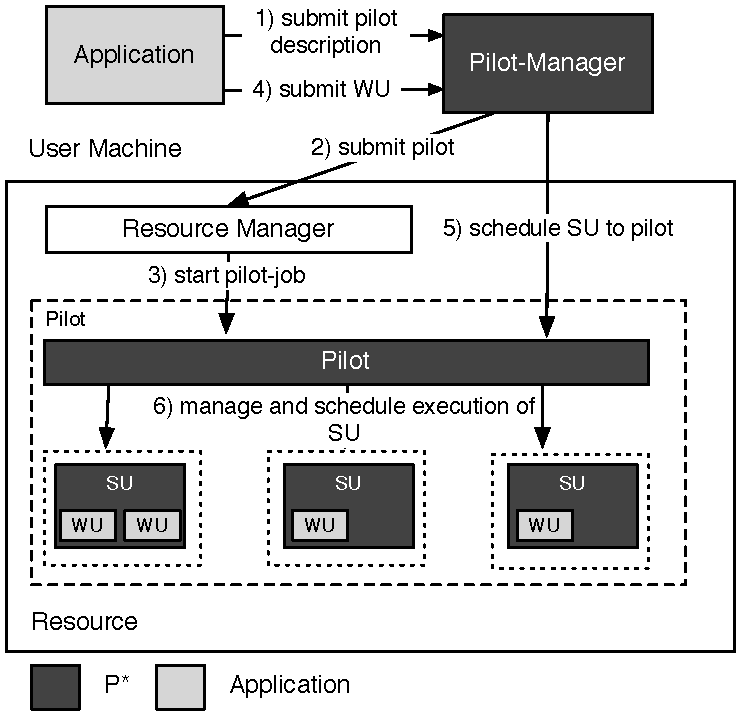
\includegraphics[width=0.45\textwidth]{figures/pstar_model_single.pdf}
    \caption{ \textbf{P* Model: Elements and Interactions:} The core
      of the model is the manager that is responsible for managing
      pilot-jobs and WUs. After a WU is submitted to the manager, it
      transitions to an SU, which is scheduled to a pilot by the PM. The pilot 
	  then schedules the SU to an available resource. \alnote{Needs
        simplification. Further we need to agree somehow on i) how
        many layers of binding/scheduling? ii) the usage of
        submit/assign/bind/schedule} \jhanote{Should we replace
        Application Kernel with SU's of different sizes i.e.,
        different number of fixed-sized WUs?} \alnote{see proposal 
		above}\upp\upp}
    \label{fig:figures_pstar}
\end{figure}


\section{TROY: A Reference Implementation and API for the P*
  Model\upp\upp}

% \terminology{TROY (implementation), P* Model, TROY API, PJ
%   implementation, BigJob, based on SAGA, PJ description, WU
%   description, TROY manager class, Condor Glide-In, DIANE, PJ-like
%   API extension) } \alnote{Lead: MS} \alnote{Renaming section and
%   subsections: TROY: A reference implementation of the P*}

%Pilot-Abstraction for Dynamic Execution 

% \jhanote{Mark to put in a para about how the API implements different
%  Pilot-Jobs} \msnote{In hindsight not sure why it was at this place,
%  and what you expected but here is an attempt:}

% \jhanote{Need to define and motivate TROY better, i.e. TROY: BigJob +
%   BigData etc.}

% \amnote{I disagree with the term runtime environment, but that is
%   probably not very important in the context of this paper.}

TROY is an implementation of the P* Model
(\S\ref{sec:pilot-model}). It consists of the TROY API~\cite{troy_api}, a
runtime engine and a set of adaptors for various PJ frameworks (see
Figure~\ref{fig:figures_pstar_troy}). TROY is consistent with the SAGA
API. SAGA~\cite{saga_url,saga_gfd90} provides a simple, POSIX-style
API to the most common grid functions at a sufficiently high-level of
abstraction so as to be independent of the diverse and dynamic grid
environments. The TROY API itself was designed to be similar to SAGA
in appearance and philosophy: it re-uses many of the well defined and
standardized semantics and syntax of the File, Job and Advert API.
\msnote{Is this true about Advert?} A further design consideration of
TROY was a minimal but complete API.

%of we aimed for
% exposing the least
% details necessary.  

\begin{figure}[t]
	\centering
		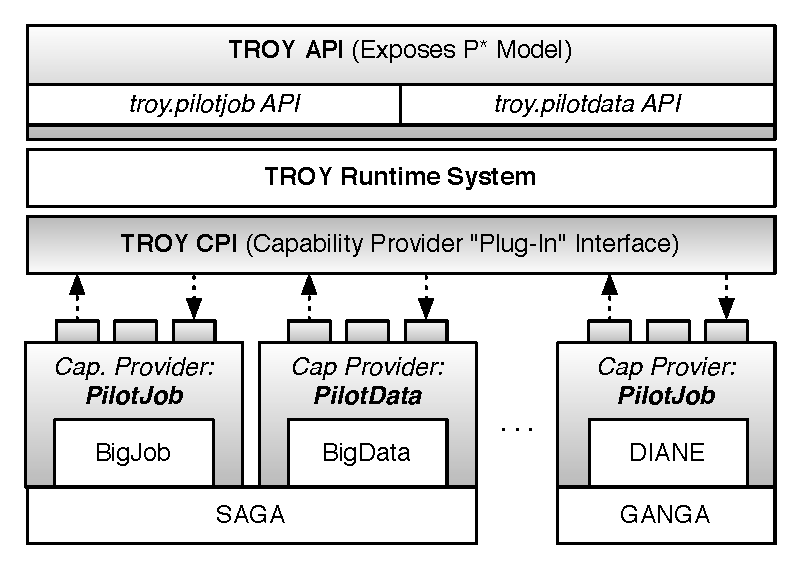
\includegraphics[width=0.45\textwidth]{figures/TROY_arch.pdf}
                \caption{\textbf{TROY -- An API and Runtime System for
                    the P* Model:} TROY provides an API for managing
                  PJs and PDs. BigJob and BigData are realizations of
                  the actual PJ and PD functionality. BJ and BD rely
                  on SAGA for implementation of the PJ/PD.\alnote{We
                    are using the term Capability Provider and Adaptor
                    interchangeably. Should we make fig 2 \& 3
                    consistent? Also, we need to be consistent with
                    this respect in our writing in sec III.}  }
	\label{fig:figures_pstar_troy}
\end{figure}

Figure~\ref{fig:figures_troy_classes} displays the main classes that
make up the Python implementation of TROY.  Although there is no
one-to-one mapping of elements of the P* model to classes, the
implementation does offer the expressiveness that the P* model aims
at. \alnote{I think we should to try to explicitly map things: WU ==
  WU, SU == SU, resource assignment: step 1-3 in fig1 =
  PilotJobService, Workload submission: step 4-6 = WorkUnitService,
  PilotJobService/WorkUnitService == PilotManager, Pilot == handled
  within the PJ framework?}  Like the P* model, the TROY API aims to
decouple workload management and resource scheduling by exposing two
separate services to the application.  The Pilot Job Service is used
for creating, managing, querying and canceling of pilot-jobs while the
Work Unit Service is responsible for managing the execution of Work
Units for the application. \alnote{How should we spell Pilot Job
  Service? Pilot Job Service? As the class name PilotJobService?
  pilot-job service? ...} In the spirit of SAGA, the instantiation of
pilot-jobs and work units is done by creating a description and
passing that to a service responsible for the creation of the
instance. The description can be reused and has no state, while the
instance has state and is a reference for further usage.

The TROY adaptors that implement the Capability Provider Interface
(CPI) provide access to the underlying pilot-job frameworks. The heart
of the engine is formed by the scheduler that maps the work units to
the internal scheduling units.  \alnote{Would it make sense to include
  the CPI and engine in the class diagram?}  These scheduling units
are not exposed to the application.

\begin{figure}[t]
	\centering
		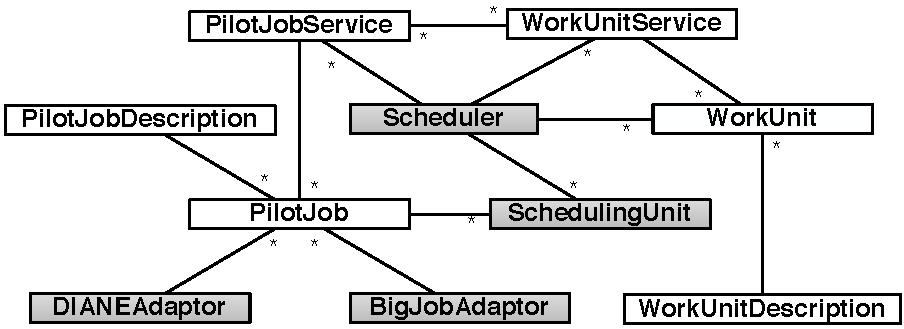
\includegraphics[width=0.47\textwidth]{figures/troy_classes.pdf}
                \caption{\textbf{TROY Class Diagram:} The classes used
                  in the TROY implementation. Classes that are not
                  exposed to the application are greyed out and
                  cardinality is shown between classes.  }
	\label{fig:figures_troy_classes}
\end{figure}

Also shown in figure~\ref{fig:figures_troy_classes} is the cardinality between
the classes. An application can have any number of Pilot Job Services or Work
Unit Services. Multiple Pilot Job Services can be associated to a Work Unit
Service, and a Pilot Job Service can be associated to multiple Work Unit
Services. A Work Unit Service can manage multiple Work Units, but a Work Unit
can only be managed by one Work Unit Service. So can a Work Unit Service manage
multiple pilot-jobs, but can a pilot-job only be managed by one Pilot Job
Service.

In figure~\ref{fig:figures_troy_flow} the flow of a simple execution scenario is
displayed. The Pilot Job Service and the Work Unit Service are already
instantiated. The application requests the Pilot Job Service to create a new
pilot-job (step 1), the Pilot Job Service will pass the request on to the
relevant adaptor (step 2) which will eventually launch the pilot-job on a
resource using a pilot-job framework (step 3). At this stage there might be a
pilot-job already available, or the request can still reside in a queue
somewhere. Regardless of the state of the pilot-job, the application can submit
a work unit to the Work Unit Service (step 4). The Work Unit Service remains
responsible for keeping track of the Work Unit during its lifetime. It will
schedule the Work Unit to the Scheduler (step 5). Based on the scheduling
policies the scheduler will decide on the mapping from Work Unit to Scheduling
Unit and will eventually schedule a Scheduling Unit to an Adaptor (step 6). 
\alnote{I thought a WU transitions to a SU at the boundary of the API?}
Finally the adaptor will submit the Scheduling Unit to the pilot-job framework
which will take care of the actual execution on a resource. \alnote{should we 
add a some remarks about the multiple levels of scheduling that are going on:
1) TROY-level scheduling vs. 2) PJ framework level scheduling?} \alnote{also 
some notes on the P* characteristics: communication, coordination would be 
good.}

To further illustrate the TROY API we include three short code snippets that 
together form a complete Python application (modulo imports).

\lstset{
language=Python,
caption={Instantiate a Pilot Job Service and Pilot Job Description, populate it 
with requirements and create a Pilot Job of type BigJob from 
it.\label{lst:pjs_creation}},
frame=single,
captionpos=b,
stringstyle=\ttfamily,
basicstyle=\scriptsize\ttfamily
}
\noindent\begin{minipage}{0.47 \textwidth}
\begin{lstlisting}
pjs = PilotJobService()
pj_desc = PilotJobDescription()
pj_desc.total_core_count = 8
pj = pjs.create('gram://queenbee', pj_desc, 'bigjob')
\end{lstlisting}
\end{minipage}

\lstset{
caption={Instantiate a Work Unit Service and associate a Pilot Job Service with it.\label{lst:wus_reation}},
}
\noindent\begin{minipage}{0.47 \textwidth}
\begin{lstlisting}
wus = WorkUnitService()
wus.add(pjs)
\end{lstlisting}
\end{minipage}

\lstset{
caption={Instantiate a Work Unit Description, populate it with application parameters submit it through the Work Unit Service.\label{lst:wu_submission}},
}
\noindent\begin{minipage}{0.47 \textwidth}
\begin{lstlisting}
wu_desc = WorkUnitDescription()
wu_desc.executable = '/bin/bfast'
wu_desc.arguments = ['match', '-t4', '/data/file1']
wu_desc.total_core_count = 4
wu = wus.submit(wu_desc)
\end{lstlisting}
\end{minipage}

The TROY API renders the artifacts defined by the P* model, as defined in
\S\ref{sec:pilot-model}. It defines two description classes that extend SAGA's
Job Description: the PJ description and the WU description. A TROY manager class
represents a pool of resources -- resources can be added by submitting a PJ
description to the TROY manager, using the \texttt{add\_resource()} method.
Subsequently, WUs can be submitted to the TROY manager. Resources can be added
and removed at any time (i.e. at runtime). TROY supports different usage modes
i) it provides a unified API to various PJ frameworks (e.\,g.\ BigJob,
DIANE and Condor-G), and ii) it enables the concurrent usage of multiple PJ
implementations. 
% Further, we show in section~\ref{sec:bigdata} how TROY is
% extended to support dynamic data and affinity-based scheduling.



\begin{figure}[t]
	\centering
		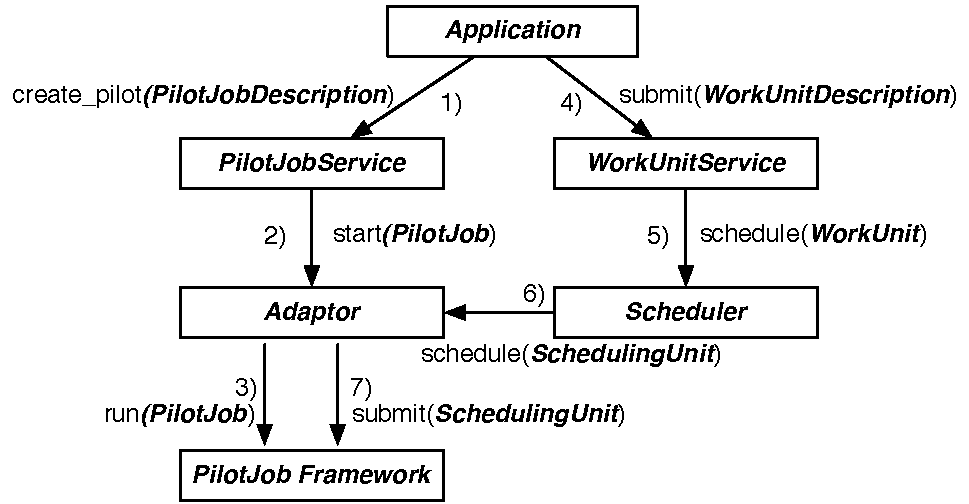
\includegraphics[width=0.47\textwidth]{figures/troy_flow.pdf}
	\caption{\textbf{TROY Flow Diagram:} The flow for the starting of a 
	pilot-job and the execution of a work unit.
	}
	\label{fig:figures_troy_flow}
\end{figure}
% \begin{figure}[htbp]
% 	\centering
% 		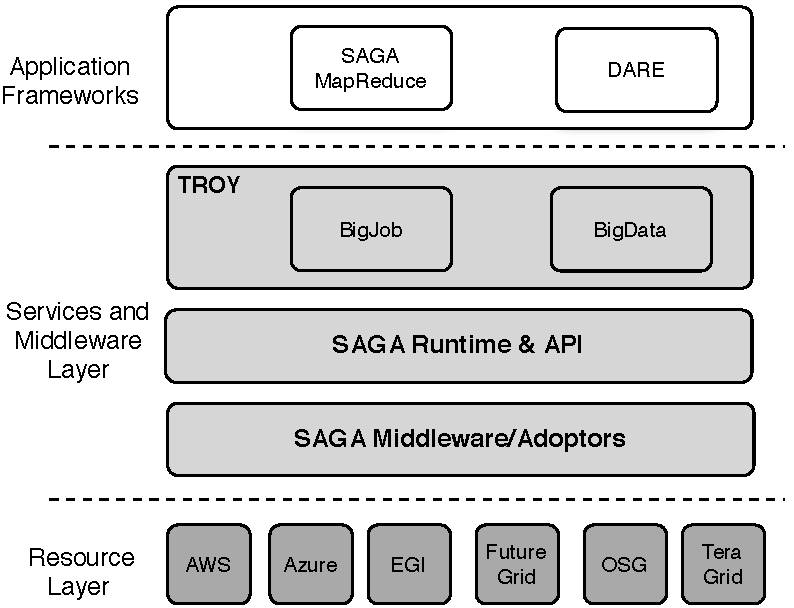
\includegraphics[width=0.45\textwidth]{figures/troy.pdf}
% 	\caption{TROY Overview}
% 	\label{fig:figures_troy}
% \end{figure}

The SAGA inspired approach to TROY's API design, and its also SAGA
inspired adaptor based architecture, leverage on the design
experiences of SAGA, and seems to appeal our pilot-job user community.
Also, the chosen designs allow to very easily exchange the actual PJ
implementation and to concurrently use multiple PJ frameworks, as
will be shown below.  TROY thus functions as common access layer for
different PJ frameworks, providing interoperability and
portability of PJ applications.  To some extent, the TROY API can be
considered to be a prototype of a PJ-like API extension to SAGA (see
future work, \S{VI}).


\section{Pilot-Jobs Frameworks\upp\upp}
\alnote{add cross-cutting analysis}

As more applications take advantage of dynamic execution, the
Pilot-Job concept has grown in popularity and has been extensively
researched and implemented for different usage scenarios and
infrastructure. There is a variety of PJ frameworks:
Condor-G~\cite{condor-g}, SWIFT~\cite{Wilde2011},
DIANE~\cite{Moscicki:908910}, DIRAC~\cite{1742-6596-219-6-062049},
PanDA~\cite{1742-6596-219-6-062041}, ToPoS~\cite{topos},
Nimrod/G~\cite{10.1109/HPC.2000.846563}, Falkon~\cite{1362680} and
MyCluster~\cite{1652061} to name a few. The aim of this section is to
show that our P* Model can be used to explain/understand some of these
PJ frameworks, in particular BigJob, DIANE as well as Condor-G and
Swift.  Table~\ref{table:bigjob-saga-diane} shows how the elements P*
model can be mapped to these
frameworks. Table~\ref{table:pilot-job-comparison} compares the
characteristics of the four PJ frameworks.

\alnote{Should we somewhere explain how these framework work together with TROY? 
We do this at least in the BJ case.}

\subsection{BigJob: A SAGA-based Pilot-Job Implementation for
  TROY\upp\upp}
\terminology{BigJob (BJ) , BigJob-SAGA, BJ implementation,  BJ-SAGA, BJ flavors, Amazon EC2, Microsoft Azure,
 BJ with a Condor Glide-In based backend,  BigJob Manager, BigJob agent component, BigJob framework,
 BigJob pool, extensible scheduler, } 


% \jhanote{MUST provide SAGA URL for updated BigJob API and
%   documentation}

% \jhanote{Alternative title: ``BigJob: TROY Pilot-Job'' ?}

% \jhanote{It is CRITICAL to explain why we need to expose the details
%   of multiple atomic BigJobs to the end-user? Remember part of the
%   whole idea of the exercise is, (i) theory: to provide a framework
%   for understanding any differences, (ii) practice: make all these
%   differences go away from the end user!}  \alnote{Since we were not
%   sure about the term ``atomic'', we could also use base bigjob, or
%   core bigjob}



   % 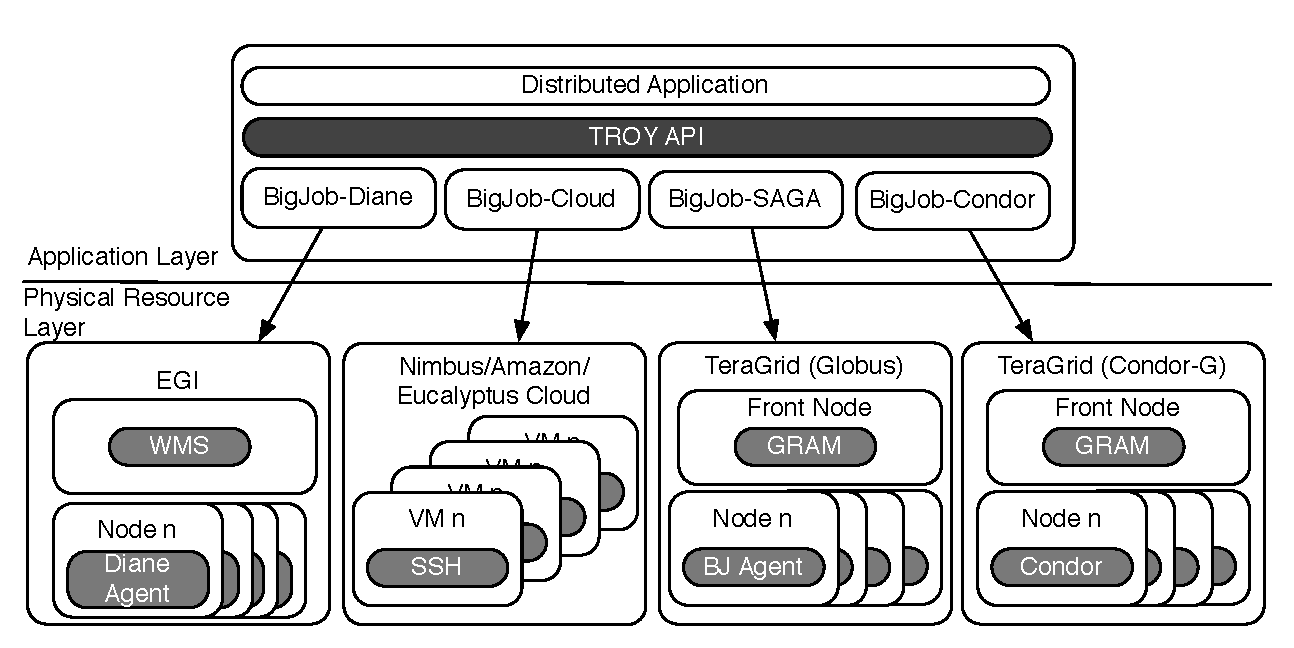
\includegraphics[width=0.3\textwidth]{figures/distributed_pilot_job.pdf}
    % 	\caption{SAGA-based TROY Implementation - BigJob}
    % 	\label{fig:figures_distributed_pilot_job}
    % 	\end{figure}


% General overview of BJ implementations & P* model
%PJ implementations in TROY are called BigJob (BJ)~\cite{bigjob_web}.
BigJob (BJ)~\cite{bigjob_web,saga_bigjob_condor_cloud} is a SAGA-based pilot-job
implementation. BJ supports a wide range of application types, and is usable
over a broad range of infrastructures, i.\,e.\ it is general-purpose and
extensible. BJ is integrated into the TROY runtime environment via the described
adaptor mechanism (see Figure~\ref{fig:figures_distributed_pilot_job}). In
addition there are specific BJ flavors for cloud resources such as Amazon EC2
and Microsoft Azure that are capable of managing set of VMs, as well as a BJ
with a Condor-G based backend. 

\begin{figure}[t]
    \centering
    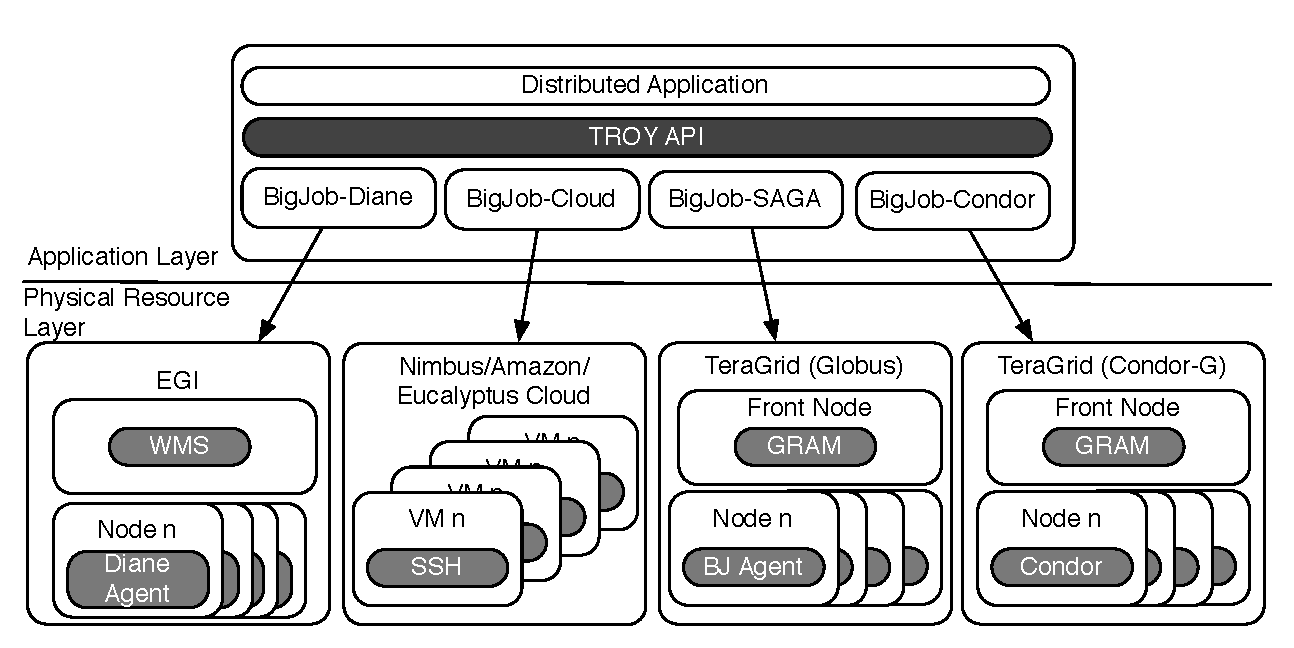
\includegraphics[width=0.48\textwidth]{figures/distributed_pilot_job.pdf}
    \caption{\textbf{BigJob -- A SAGA-based Pilot-Job Implementation:}
      BigJob is the implementation of the actual PJ functionality for
      TROY. Further, TROY integrates with various other PJ frameworks
      providing pilot-job capabilities on different types of
      distributed infrastructures. SAGA BigJob permits usage with
      multiple middleware backends~\cite{saga_bigjob_condor_cloud} }
    \label{fig:figures_distributed_pilot_job}
\end{figure}

% In the scope of this paper, BJ generally refers
% to the BJ-SAGA implementation though.

BJ utilizes a M/W coordination model: The BigJob Manager is responsible for the
orchestration of pilots, for the binding of WUs and for the scheduling of SUs.
For submission of the pilots, SAGA relies on the SAGA Job API, and thus can be
used in conjunction with different SAGA adaptors, e.\,g.\ the Globus, PBS,
Condor Amazon Web Service and other adaptors. Each pilot initializes a so called
BigJob agent. The agent is responsible for gathering local information and for
executing tasks (SUs) on its local resource. The SAGA Advert Service API is used
for communication between manager and agent. The Advert Service (AS) exposes a
shared data space that can be accessed by manager and agent, which use the AS to
realize a push/pull communication pattern, i.\,e.\ the manager pushes a SU to
the AS while the agents periodically pull for new SUs. Results and state updates
are similarly pushed back from the agent to the manager. Further, BJ provides a
pluggable communication \& coordination layer and also supports alternative c\&c
systems, e.\,g.\ Redis~\cite{redis} and ZeroMQ~\cite{zmq}.

BJ currently uses a simple binding mechanism: each WU (a task)
submitted to the BigJob framework is mapped to one SU (a so called
sub-job).  Binding takes places at submission time (early binding).
For scheduling, a simple FIFO scheduler is used (see also
Table~\ref{table:pilot-job-comparison}).


% All core BJ are confined to a single resource and don't allow
% neither elasticity nor late binding.

%paragraph on dynamic capabilities

In many scenarios it is beneficial to utilize multiple resources, e.\,g.\ to
accelerate the time-to-completion or to provide resilience to resource failures
and/or unexpected delays. The TROY API allows for dynamic resource
additions/removals as well as late binding. The support of this feature depends
on the backend used. To support this feature on top of various BigJob
implementations that are by default restricted to single resource use (e.\,g.\
BJ), the concept of a BigJob pool is introduced. A BigJob pool consists of
multiple BJs (each BigJob managing one particular resource). An extensible
scheduler is used for dispatching WUs to one of the BJs of the pool (late
binding). By default a FIFO scheduler is provided. Other backends (such as DIANE
and Condor) natively support elasticity, but can nevertheless be combined into a
BJ pool.

% \input{sectionIV_comments}
\upp

\begin{table*}[t]
\centering
\begin{tabular}{|p{2.5cm}|p{3cm}|p{3cm}|p{3cm}|p{3cm}|}
\hline
\textbf{P* Element} &\textbf{BigJob} &\textbf{DIANE} &\textbf{Condor-G} &\textbf{Swift-Coaster}  \\
\hline
Manager &BigJob Manager & RunMaster & condor\_master, condor\_collector, condor\_negotiator, condor\_schedd &Coaster Service\\ 
\hline
Pilot-Job &BigJob Agent  & Worker Agent &condor\_master, condor\_startd &Coaster Worker\\
\hline
Unit of Work &Task &Task &Job &Application Interface Function (Swift Script)\\
\hline
Unit of Scheduling &Sub-Job &Task &Job &Job\\
% \hline
% Dynamic Resources &no/yes &yes (AgentFactories)\\
\hline
\end{tabular}
\caption{P* Elements and Pilot-Job Frameworks\up} \label{table:bigjob-saga-diane}
\end{table*}

\upp
\subsection{DIANE\upp\upp}

% Coordination and Communication
DIANE~\cite{Moscicki:908910} is a task coordination framework, which was
originally designed for implementing master/worker applications, but also
provides PJ functionality for job-style executions. DIANE utilizes a single
hierarchy of worker agents as well as a PJ manager referred to as
\texttt{RunMaster}.
%Further, there is ongoing work on a multi-master extension.
For the spawning of PJs a separate script, the so-called submitter script, is
required. For the access to the physical resources the GANGA
framework~\cite{DBLP:journals/corr/abs-0902-2685} can be used.
%GANGA provides a
%unified interface for job submissions to various resource types, e.\,g.\ EGI
%resources or TG resources via a SAGA backend.
Once the worker agents are started they register themselves at the RunMaster.
In contrast to TROY-BigJob, a worker agent generally manages only a single
core and thus, by default is not able to run parallel applications (e.\,g.\
based on MPI). BJ utilizes the BJ agent that is able manage a set of local
resources (e.\,g.\ a certain number of nodes and cores) and thus, is capable
of running parallel applications. For communication between the RunMaster and
worker agents point-to-point messaging based on CORBA~\cite{OMG-CORBA303:2004}
is used. CORBA is also used for file staging, which is not fully supported by
BJ, yet.

% Binding 
DIANE is primarily designed with respect to HTC environments (such as
EGI~\cite{egi}), i.\,e.\ one PJ consists of a single worker agent with the
size of 1 core. BJ in contrast is designed for HPC systems such as TG,
where a job usually allocates multiple nodes and cores. To address this issue
a so-called multinode submitter script can be used: the scripts starts a
defined number of worker agents on a certain resource. However, WUs will be
constrained to the specific number of cores managed by a worker agent. A
flexible allocation of resource chunks as with BJ is not possible. By
default a WU is mapped to a SU; application can however implement smarter
allocation schemes, e.\,g.\ the clustering of multiple WUs into a SU.

%Scheduling
DIANE includes a simple capability matcher and FIFO-based task scheduler.
Plugins for other workloads, e.\,g.\ DAGs or for data-intensive
application, exist or are under development. The framework is extensible:
applications can implement a custom application-level scheduler.


%Other impl. related issues: FT and security
DIANE is as BJ a single-user PJ, i.\,e.\ each PJ is executed with the
privileges of the respective user. Also, only WUs of this respective user can be
executed by DIANE. DIANE supports various middleware security mechanisms
(e.\,g.\ GSI, X509 authentication). For this purpose it relies on GANGA. The
implementation of GSI on TCP-level is possible, but currently not yet
implemented. Further, DIANE supports fault tolerance: basic error detection and
propagation mechanisms are in place. Further, an automatic re-execution of WUs
is possible.

\upp
\subsection{Condor-G\upp\upp}

Condor-G pioneered the Pilot-Job concept~\cite{condor-g}. The pilot is
actually a complete Condor pool that is started using the Globus service of a
resource. This mechanism is referred to as Condor Glide-In. Subsequently, jobs can be submitted to this Glide-In pool using the
standard Condor tools and APIs. Condor utilizes a master/worker coordination
model. The PJ manager is referred to as the Condor Central Manager. The
functionality of the Central Manager is provided by several daemons: the
condor\_master that is generally responsible for managing all daemons on a
machine, the condor\_collector which collects resource information, the
condor\_negotiator that does the matchmaking and the condor\_schedd that is
responsible for managing the binding and scheduling process. Condor generally
does not differentiate between workload, i.\,e.\ WU, and schedulable entity,
i.\,e.\ SU. Both entities are referred to as job. However, it supports late
binding, i.\,e.\ resources a job is submitted to must generally not be available
at submission time. The scheduler matches the capabilities required by a WU to
the available resources. This process is referred to as matchmaking. Further, a
priority-based scheduler is used. For communication between the identified
elements Condor utilizes point-to-point messaging using a binary protocol on top
of TCP.

Different fault tolerance mechanisms, such as automatic retries, are supported.
Further, Condor supports different security mechanisms: for authentication it
integrates both with local account management systems (such as Kerberos) as well
as grid authentication systems such as GIS. Communication traffic can be
encrypted.


\upp
\subsection{SWIFT-Coaster\upp\upp}

SWIFT~\cite{Wilde2011} is a scripting language designed for expressing abstract
workflows and computations. The language provides among many things capabilities
for executing external application as well as the implicit management of data
flows between application tasks. For this purpose, SWIFT formalizes the way that
applications can define data-dependencies. Using so called mappers, these
dependencies can be easily extended to files or groups of files. The runtime
environment handles the allocation of resources and the spawning of the compute
tasks. Both data- and execution management capabilities are provided via
abstract interfaces. SWIFT supports e.\,g.\ Globus, Condor and PBS resources.
The pool of resources that is used for an application is statically defined in a
configuration file. While this configuration file can refer to highly dynamic
resources (such as OSG resources), there is no possibility to manage this
resource pool programmatically. By default a 1:1 mapping for WU and jobs is
used. However, SWIFT supports the grouping SUs as well as PJs. For the PJ
functionality the Coaster~\cite{coasters} framework is used. Coaster relies on a
master/worker coordination model; communication is implemented using GSI-secured
TCP sockets. SWIFT and Coaster supports various scheduling mechanisms, e.\,g.\ 
a FIFO and a load-aware scheduler. 

Further, SWIFT can be used in conjunction with Falkon~\cite{1362680}. Falkon
refers to pilots as the so called provisioner, which are created using the
Globus GRAM service. The provisioner spawns a set of executor processes on the
allocated resources, which are then responsible for managing the execution of
SUs. WUs are submitted via a so called dispatcher service. Similar to Coaster,
Falkon utilizes a M/W coordination model, i.\,e.\ the executors periodically
query the dispatcher for new SUs. Web services are used for communication.



% \jhanote{It should probably be Coasters -- which is their notion of a
%   pilot-job.  Just to keep life interesting, they call it head-job and
%   not pilot-job!
%   \url{http://www.ci.uchicago.edu/swift/guides/release-0.92/userguide/coasters.php }}

% \alnote{SWIFT eval: no standard resource abstraction (SAGA),
%   proprietary language (not Python), TODO: check how coasters work!
%   1 coaster == 1 Condor-G job?}


%\subsubsection*{Other Pilot-Jobs and Conclusion}

% \jhanote{Can we add some structure to these *other* PJ.. this will be
%   ambitious and time-consuming, but if we can, that'll be (i) a great
%   service to the community, (ii) a strong intellectual addition to the
%   paper by virtue of validation of the P*-model}

\alnote{which are the minimal P* elements and characteristics we
  should discuss here?}  \jhanote{Andre L: Is this still a valid/live
  comment/question? If not, should we close}\alnote{can be closed.}

\begin{table*}[t]
\centering
\begin{tabular}{|l|p{2.5cm}|p{2.5cm}|p{2.5cm}|p{2.5cm}|}
	\hline
	\textbf{P* Characteristic}
	&\textbf{SAGA BigJob} &\textbf{DIANE} &\textbf{Condor-G} &   
	\textbf{SWIFT Coaster} \\ \hline
End User Environment &API &API and Master/Worker Framework &CLI Tools &Swift script\\ \hline

Coordination &Master/Worker  &Master/Worker  &Master/Worker &Master/Worker \\ \hline
	
Communication &Advert Service &CORBA &TCP &GSI-enabled TCP \\ \hline

Binding &Early/Late &Late &Late &Late\\
% \hline
% MPI/Multinode Applications &yes &no (yes with custom implementation of ApplicationWorker)\\
\hline
Scheduling &FIFO, custom &FIFO, custom &Matchmaking, priority-based scheduler 
&Load-aware scheduler, WU grouping\\
\hline

Security &Multiple (GSI, Advert DB Login) &Multiple (GSI) &Multiple (GSI, 
Kerberos) &GSI\\ \hline

Resource Abstraction &SAGA &GANGA/SAGA &Globus &Resource Provider API/Globus CoG 
Kit \\ 
\hline
Agent Submission &API &GANGA Submission Script &Condor CLI 
&Resource Provider API\\
% \hline
% Application Interfaces &Big-Job/Sub-job Management &Big-Job/Sub-job 
% Management\linebreak[4] Master/Worker API (\texttt{ITaskScheduler}, 
% \texttt{IApplicationManager}, \texttt{IApplicationWorker}) &&\\
\hline
Fault Tolerance &Error propagation &Error propagation, Retries &Error propagation, Retries &Error propagation, retries, replication\\
\hline
	
\end{tabular}
\caption{P* Characteristics and Pilot-Job Implementations\up}\label{table:pilot-job-comparison}
\end{table*}

\upp
\section{Experiments and Results\upp\upp}
% In this section we discuss the TROY API. Further, (i) we show that the TROY API
% can be used to marshal DIANE stand-alone as well as (ii) that the TROY API can
% be used stand alone with both BigJob and DIANE concurrently. 

\jhanote{MS: The experiment section needs tighter and more focussed
  writing in general}

In this section we analyze the performance and scalability of different PJ
implementations in particular of BigJob and DIANE. Further, we investigate PJ
framework interoperability by using TROY in conjunction with different TROY 
adaptors. For this purpose we deploy TROY with BigJob (with SAGA/PBS and 
SAGA/Condor) and DIANE in a genome sequencing application scenario. The 
experiments are conducted on different production (LONI, OSG) and research
infrastructures (FutureGrid).

\subsection{Understanding Pilot-Job Implementations}

Each PJ implementation is associated with various degrees of freedom, in
particular in the design of the communication \& coordination (c\&c) sub-system.
The primary barrier for performance and scalability is not the WU submission,
but the internal coordination of the elements of a P* implementation. There are
many factors that influence the overall performance, e.\,g.\ the degree of
distribution (local (LAN) vs. remote (WAN)), the communication pattern (1:n
versus n:n) and the communication frequency. In the following we investigate the
impact of different c\&c related factors on the overall performance and
scalability of the system.

The original design of BigJob is based on a shared, centralized data space, the
SAGA Advert Service~\cite{saga_advert}, which is essentially a PostgreSQL
database. The communication between all components is done via this data space;
this concept is also known as tuple space~\cite{Gelernter:1985:GCL:2363.2433}.
The data space decouples BJ manager and BJ agent very well and allows both
entities to operate at their own pace optimizing the overall throughput.
Depending on the setup this data space can be deployed locally, i.\,e.\ on the
same resource, or remotely, e.\,g.\ during a distributed run. A particular issue
during distributed runs is the latency between the application and the Advert
Service. Another challenge is that this design introduces a potential
single-point-of-failure and scalability bottleneck if the centralized data space
is not carefully designed and operated. 


BigJob also provides two alternative c\&c sub-systems: Redis~\cite{redis} and ZeroMQ~\cite{zmq}. Redis is a lightweight key/value store, which can
be deployed in a distributed, fault tolerant way. Redis is used in a similar way
as the Advert database, i.\,e.\ all communication between BJ agent and manager
is channeled through it. Redis can be deployed locally and remotely. 
The ZeroMQ c\&c sub-system in contrast utilizes a client-server
architecture, which is similar to the CORBA-based~\cite{OMG-CORBA303:2004} 
communication system of DIANE. In this architecture, the PM maintains the 
overall state. Clients connect to the
PM to request new SUs or to report state updates. An advantage of this
architecture is that it does not require a separate infrastructure for
deployment of the Advert Service or the Redis database. While the BJ manager can
be deployed remotely from the BJ agent, in most cases this will not be the case,
i.\,e.\ the communication between BJ manager and BJ agent is mostly local
communication. Both the data space and client-server c\&c sub-system can be
combined with a publish/subscribe mechanisms, i.\,e.\ instead of polling an
agent or client can receive notifications when a new SU arrives. In the
following, we evaluate different BJ configurations and compare and contrast them
with DIANE. For this purpose, we conducted several experiments on
FutureGrid~\cite{fg}. To evaluate the overall performance and throughput, we
execute a different number of WUs on Alamo and Sierra
utilizing up to 128 cores concurrently. 



\jhanote{Need to motivate testing of c\&c sub-system better: There are
  many barriers to interoperability and performance. primary barrier to
  performance is not WU submission or SU scheduling to PM, but the
  fundamental limitation of scalability of coordination -- with
  increasing number of WU/SU.  Establish tradeoff between distributed
  vs local coordination. e.g., It is easy to get consistency but has
  overhead.  Easy to get performance but difficult to get
  consistency. Thus we opt for centralized / persistent point. But how
  does this single point-of-coordination behave with increasing number
  of connections? } \alnote{hopefully addressed most points in paragraph above}

% \begin{figure*}[htbp]
% 	\centering		
% 	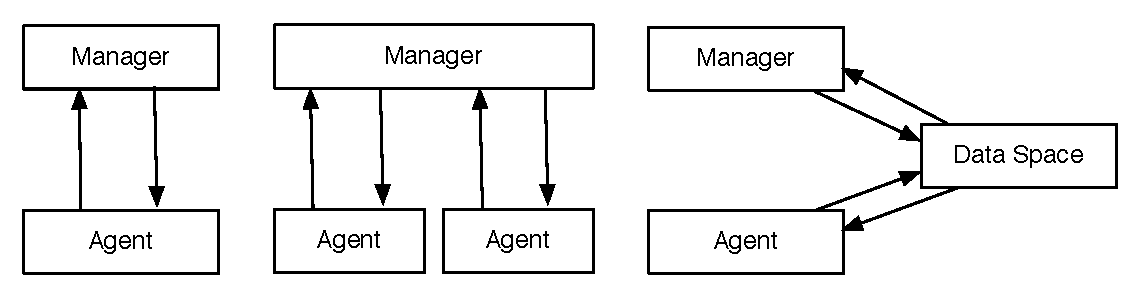
\includegraphics[width=0.8\textwidth]{figures/coordination-schemes.pdf}
% 	\caption{\textbf{Coordination \& Communication:} The primarily used 
% 	coordination pattern is the utilization of a request/response server 
% 	(left, middle). In the data-space model (right) all application components 
% 	are connect to a central data-space. This architecture decouples manager 
% 	and agent allowing both to operate on its own pace.}
% 	\label{fig:figures_coordination-schemes}
% \end{figure*}

% Figure~\ref{fig:figures_coordination-schemes} illustrates different
% coordination schemes. 

% Most pilot-jobs utilize the master-worker \jhanote{M-W for what?}
% pattern commonly implemented on basis of a simple request/response
% architecture, i.\,e.\ the \jwave{agent} sends a request for work
% packages to the master, which replies with a WU. 
\jhanote{Are we talking specific implementation, i.e., TROY? If so we
  should not say ``A'' manager but ``The Pilot-Manager''? Also the previous
sentence should not talk about most pilot-jobs, if we've already started
talking about TROY!!} \alnote{hopefully fixed.} 

% A manager
% can manage a single agent (e.\,g.\ BigJob) or multiple agents
% (e.\,g.\ DIANE). 


\begin{figure}[htbp] \centering
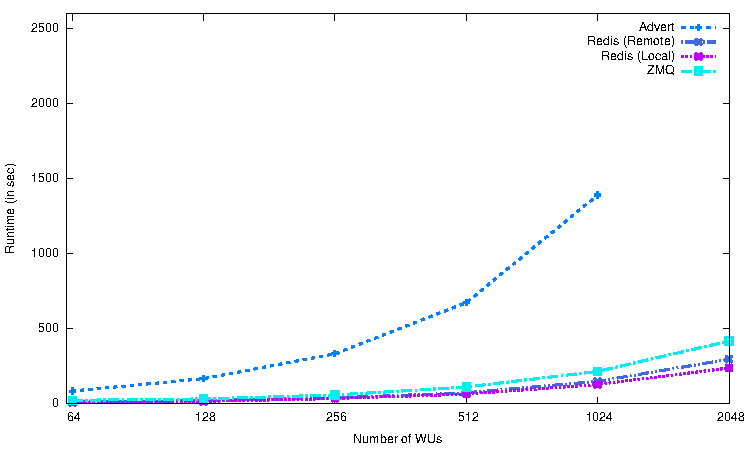
\includegraphics[width=0.49\textwidth]{perf/bigjob-varying-wus-alamo.pdf}
\caption{\textbf{BigJob and DIANE Performance (1):} The 
time-to-completion for $n$ WUs running \texttt{/bin/date} scales linearly
in most cases, i.\,e.\ the coordination overhead imposed by the BJ is 
minimal. }
\label{fig:perf_bigjob-varying-wus} \end{figure}

Figure~\ref{fig:perf_bigjob-varying-wus} illustrate the performance and
scalability of the different BigJob configurations and DIANE with respect to the
number of WUs. Clearly, the used c\&c sub-system has a great impact on the
overall performance. The Redis backend shows the best performance for small WU
counts. The difference between local and remote coordination is moderate (about
20\,\%). While ZeroMQ is very fast and lightweight, it requires a careful
implementation in particular concerning synchronization and throughput
optimization. The overall performance is slightly worse than for Redis. The
Advert Service currently has some limitations which will be discussed later.
DIANE shows a higher startup overhead, which is particularly observable for
smaller WU numbers. However, the runtime increases only slightly (about 10\,sec)
when going from 64 to 2048 WUs. A reason for this behavior is that DIANE
aggregates SUs: for 2048 WUs only a single task description is created, which
the framework then efficiently distribute to its worker agents. BigJob in
contrast maintains for each WU a separate description. 
% At the investigated
% scales, the single manager does not represent a bottleneck with respect to the
% processable WU numbers. Further, the TROY manager introduces another 
% hierarchy-level which can further
% enhance the overall scalability.

Figure~\ref{fig:perf_bigjob-varying-cores} illustrates the performance
scalability with respect to the number of cores. In particular, the Redis
(Local) configuration show an almost linear scalability up to 128 cores. The
Redis remote setup again imposed some overhead (about 14\,\%). ZeroMQ performs
very well with lower core counts; with larger core counts the runtimes increase
indicating a potential scalability bottleneck. DIANE shows in particular for
lower core counts a longer runtime again due to the higher startup overhead.
With higher core counts DIANE behaves similar to BigJob ZeroMQ showing a greater
increase of the overall runtime. This increase can likely be attributed to
the single central manager in the client-server architecture. As in the last
experiment, the Advert c\&c sub-system showed a significantly lower performance.

\begin{figure}[htbp] \centering
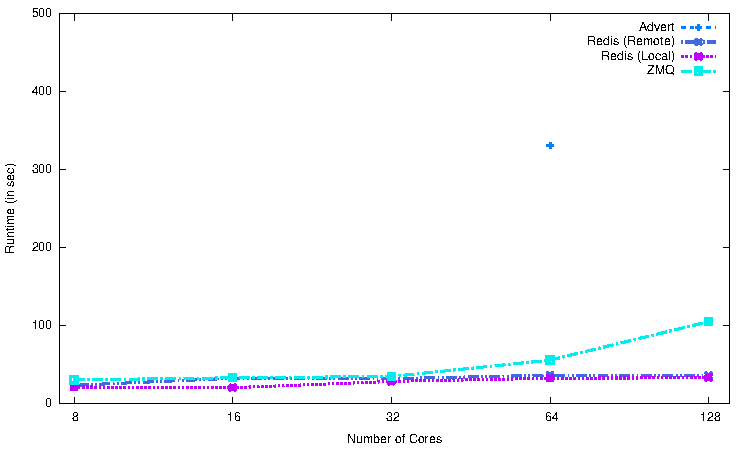
\includegraphics[width=0.49\textwidth]{perf/bigjob-varying-cores-alamo.pdf}
\caption{\textbf{BigJob and DIANE Performance (2):}  The
runtime of a constant workload of 4 \texttt{/bin/date} jobs 
increases only slightly up to 128 cores. In particular, the Redis backend shows
an almost linear scalability achieving a throughput of up to 4 WUs/sec. }
\label{fig:perf_bigjob-varying-cores} \end{figure}

The BigJob Advert implementation currently shows some performance limitations
mainly caused by the prototypical nature of the Advert Service implementation.
Further, it must be noted that the Advert Service was deployed remotely (mainly
due to deployment constraints). However, even considering this aspect the
discrepancy between Advert Service and Redis (Remote), which has been deployed
on the same remote network, is significant. A reason for the worse performance 
is the used remote access protocol. The Advert Service is based on
PostgreSQL; in the current architecture the client, i.\,e.\ the BJ
manager and agent access the PostgreSQL database via the SOCI backend
library. While this architecture provides a very flexible remote
access to the database, running database access protocol over a WAN
connection is not optimal. \jhanote{It is not clear why REDIS and
  ZeroMQ are not susceptible to access over WAN delays/latency?}\alnote{included a comparison note to Redis Remote. We can't compare it to ZMQ since we use only
local communication in this case}
Transactions e.\,g.\ are very latency sensitive and require several
roundtrips.  Further, the API is based on a hierarchical namespace,
which does not naturally map well to relational databases. In
particular deeply nested namespaces exhibit an insufficient query and
update performance. In contrast, both in the Redis and ZeroMQ scenario, data is 
stored in memory, which also explains to significant performance gains.


\subsection{Understanding TROY Interoperability}

To validate the abstractions developed, we conducted a series of experiments. We
execute BFAST~\cite{bfast2009} -- a genome sequencing application -- using TROY
in conjunction with different PJ frameworks and infrastructures. For this
purpose we deploy TROY with various BigJob configurations and DIANE. TROY-BigJob
is used with the SAGA-Globus adaptor to access LONI resources and with
SAGA-Condor adaptor to access OSG resources. Further, we utilize TROY-DIANE on
LONI. On LONI~\cite{loni} the Oliver machine and a total of 16 cores distributed
across four nodes is used, on OSG the RENCI Condor cluster is utilized.
\alnote{Sharath please fill in details} To manage the workflow we use the
DARE~\cite{dare-tg11-gateways} framework that has been built on top of TROY.

The following experimental setup is used:  Dare is used to define eight WUs for 
executing a BFAST sequence alignment configuration. We run the experiments in 
three different setups: (i) TROY-BigJob/Globus only, (ii) TROY-BigJob/Condor 
only, (iii) TROY-DIANE only and (iv)  TROY-BigJob and TROY-DIANE concurrently. 
In case (iv) on each backend four WUs are executed.


While BigJob utilizes one BJ agent on the resource, DIANE currently requires the
spawning of one worker agent per WU that must be executed in parallel. The TROY
API marshals these differences, i.\,e.\ while the API remains the same for both
backends, the different semantics in the PJ frameworks are handled by the TROY
backend.
\jhanote{What are we trying to say here?  Is it that although the API
  is similar, semantics of implementation and execution remain
  different, and that TROY backend handles them?}\alnote{well said}

Each BFAST application-kernel requires two cores; a total of eight WUs
allocating two cores each is specified and assigned to TROY. Each WU
is associated with a set of input files. After submission of the WU to
the PJ manager, the TROY runtime takes care of binding and scheduling
the WUs to the pilots. The application can monitor the state of the
PJs and WUs using the TROY API.


% To perform the above experiments we built an application \smnote{this
% application is DARE. do we need mention it here?} using TROY API to submit Bfast
% WU's with different input files to different backend implementations. The WU's
% are completely handled and submitted to different backends by TROY and the
% co-ordination of WU's was made simple for the application. Further, applications
% can also continuously monitor status of remote agents and UOWs.

% Further, it shows that both PJ implementations can be used
% concurrently. This is particularly useful if the time-to-completion can be
% reduced in cases where resources on another infrastructure are available.

\begin{figure}[t]
	\centering
		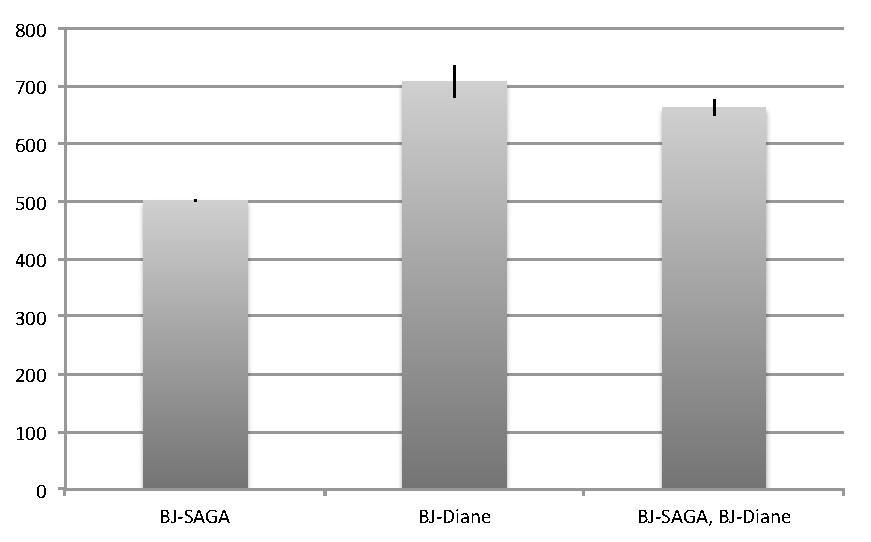
\includegraphics[width=0.4\textwidth]{perf/perf-bfast-bj.pdf}
	\caption{\textbf{Performance TROY with BigJob and DIANE:} Running BFAST 
	on a 4 node cluster with a total of 16 cores. The time-to-completion for 
	TROY-DIANE is higher than for BJ mainly due to the higher startup 
	time required and some light runtime overhead caused by the additional 
	agents required on the resource.\up\up}
	\label{fig:perf_perf-bfast-bj}
\end{figure}



Figure~\ref{fig:perf_perf-bfast-bj} shows the results of the
experiments. The time-to-completion for TROY-DIANE is about 207\,sec
longer than for TROY-SAGA. The main contributor for this increased
runtime is the deployment time required for DIANE. In a multi-node
setup multiple work agents must be used (8 in this case).  For each
worker agent DIANE must be downloaded, installed and started
separately. In total this requires about 178\,sec. Further, each DIANE
worker agent is queued as a separate job at the local resource manager
-- this contributes the the higher deviation in the measured
runtimes. Because BigJob requires a pre-run installation on each site,
it only shows a startup time of 28\,sec. Additionally, we also
observed a runtime overhead of about 17\,sec for the TROY-DIANE
scenario. This overhead is likely caused by the additional agents
required.

% % In the case of BJ-DIANE backend Multinode submitter was not used/not % yet. As
% a result it submits job request's for each node separately and there % also some
% delay between actual launch and startup time of UOW. Further, DIANE % was
% installed separately for every agent/node requested.

Finally scenario iii) demonstrates that two BJ implementations can be
utilized concurrently using the TROY API. The performance in this
scenario is slightly better than in the DIANE only case, mainly due to
the fact that only four DIANE worker agents need to be started. Also,
only half of the WUs are executed on a DIANE node and thus, show a
longer runtime. While there are some limitations in the current
TROY-DIANE implementation, the aim of this experiment is to emphasizes
the possibilities that the TROY API provides to dynamic
applications. TROY enables applications to utilize a dynamic resource
pool consisting of resources of different infrastructures, e.\,g.\ EGI
and TG/XD resources. Dynamic applications can utilize the elasticity
of the TROY resource pool e.\,g.\ to improve the time-to-completion
and/or to scale the accuracy of their computations.


% Further, TROY hides many of the complications with various pilot
% jobs like multiple node backend agents, how WU's distribution to
% various backends. Thus, this enables users of this API to
% concentrate more on designing their applications instead worrying
% about the various configurations of the pilot jobs.

\upp

\section{P* Redux: Extension of P* to a Model for Pilot-Data}
\label{sec:pilot-data}

Dynamic execution is at least equally important for data-intensive
applications: applications must cope with various challenging issues
e.\,g.\ varying data sources (such as sensors and/or other application
components), fluctuating data rates, optimizations for different
queries, data-/compute co-location etc. Thus, having defined the P*
model, we explore its extension to data.
%so as to facilitate an understanding of dynamic execution. 
This will motivate an analogous abstraction that we call
\emph{pilot-data (PD)}. \jwave{PD provides late-binding capabilities
  for data by separating the allocation of physical storage and
  application-level data units.}  Further, it provides an abstraction
for expressing and managing relationships between data units and/or
work units. These relationships are referred to as
\emph{affinities}.  %

% \jhanote{difficult to use affinity without defining it..}
% \alnote{tried to describe affinities a little bit better}

\subsubsection*{Extension of P* Model Elements to Data}

% A Pilot-Data Framework facilitates the late-binding between data units
% and physical storage resources, the so called pilot-stores.

The elements defined by P* (in section~\ref{sec:p_star_elements}) can
be extended by the following elements:

\begin{compactenum}[A.]
\item \textbf{Data Unit (DU):} DU is the base unit of data assigned by
  the application,  e.\,g.\ a data file or chunk. 
\item \textbf{Pilot-Data (PD):} PD allows the logical grouping of DUs
  and the expression of data-data affinities. This collection of files
  can be associated with an extensible set of properties. One of these
  properties is affinity. 
\item \textbf{Pilot-Store (PS):} A PS functions as a placeholder
  object that reserves the space for pilot-data objects.  By assigning
  a PD to a PS, the PD is bound to a physical resource.  A PS
  facilitates the late-binding of data and resource and is equivalent
  to the pilot-job.
\item \textbf{Pilot-Data Manager} is analogous to the PJ-Manager
  responsible for managing DU, PD and PS elements. It implements the
  different characteristics of the P* model.
\end{compactenum}
 
Note, each element has can be mapped to an element in the P* Model by
symmetry, e.g., a DU correspond to a WU in the original P* Model.

% \jhanote{PJ Model is confusing. Either it is P Model or PJ
%   Framework} \alnote{ok}

% A particular critical requirement for data-intensive application, is
% the management of affinity between DUs and also between WUs and
% DUs. Thus, Pilot-Data introduces the PD container object for
% expressing relationships between DUs. A PD corresponds to an SU in
% the \jwave{PJ model}, i.\,e.\ it is used as scheduling unit for
% internal optimizations, e.\,g.\ the grouping of DUs. Having
% instantiated a PD, it can be assigned to a PS via the PD manager. A
% PS is a placeholder reserving a certain amount of storage, i.\,e.\
% it corresponds to a pilot in the pilot-job model. By associating a
% PD to a PS the data is actually moved to the physical location
% associated with the PS. The PD manager facilitates the creation of
% PSs, schedules data movements (with respect to specified affinities)
% and manages data accesses.

\subsubsection*{Application of P* Model Characteristics to Data}

While the extensed P* Model introduces new elements, the
characteristics however, remain the same to a great extent. The
coordination characteristic describes how the elements of PD interact,
e.\,g.\ utilizing the M/W model; the communication characteristic can
be applied similarly. The scheduling characteristics must be extended
to not only meet compute requirements, but also to support common data
access patterns. The scheduling component particularly needs to
consider affinities, i.\,e.\ user-defined relationships between WUs
and/or DUs, e.\,g.\ data-data affinities exist if different DUs must
be present at the same compute element; data-compute affinities arise
if data and compute must be co-located for a computation, but their
current location is different. The decision of where to place the data
and compute is made by the scheduler based on the defined policies,
affinities, available dynamic resource information.

\subsubsection*{BigData: A SAGA-based Pilot-Data Prototype for TROY}
\label{sec:bigdata}

\begin{figure}[t]
    \centering
    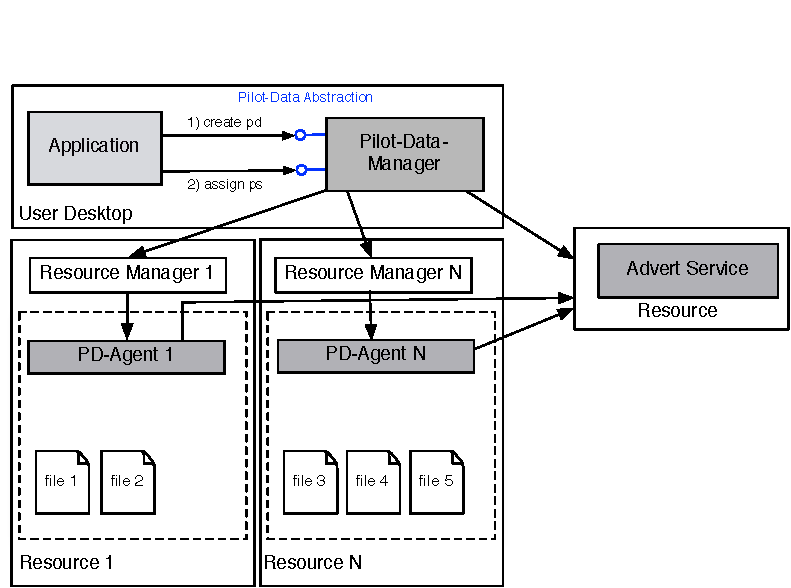
\includegraphics[width=0.48\textwidth]{figures/pilot-data-manager.pdf}
    \caption{\textbf{BigData Architecture:} The BD Manager exposes
      TROY's PD API. Application can create group of files and assign
      files to storage. The BD manager tracks file locations in the
      data catalog. The scheduler optimizes data-compute co-location.
      The transfer manager initiates and monitors data
      movements. \up\up}
    \label{fig:pilot-data-architecture}
\end{figure}

% \begin{figure*}[t]
%   \up\up\up
%   \begin{minipage}[t]{0.475\linewidth}
%     \centering
%     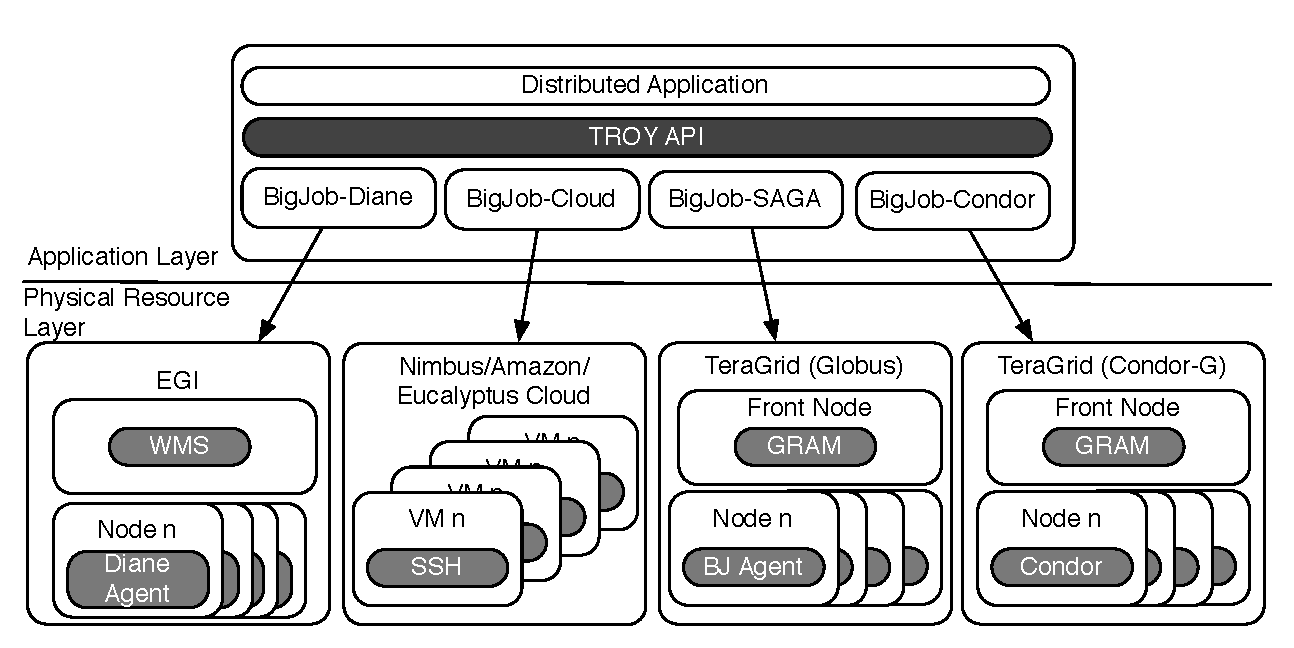
\includegraphics[width=\textwidth]{figures/distributed_pilot_job.pdf}
%     %\includegraphics[width=\textwidth]{figures/P1140340.JPG}
%     \caption{\textbf{BigJob -- SAGA-based Pilot-Job Implementation:}
%       BigJob is the implementation of the actual PJ functionality for
%       TROY. SAGA BigJob permits usage with multiple middleware
%       backends~\cite{}}
%     \label{fig:figures_distributed_pilot_job}
%     \end{minipage}
%   \hspace{0.035\linewidth}
%   \begin{minipage}[t]{0.475\linewidth}
%     \centering
%     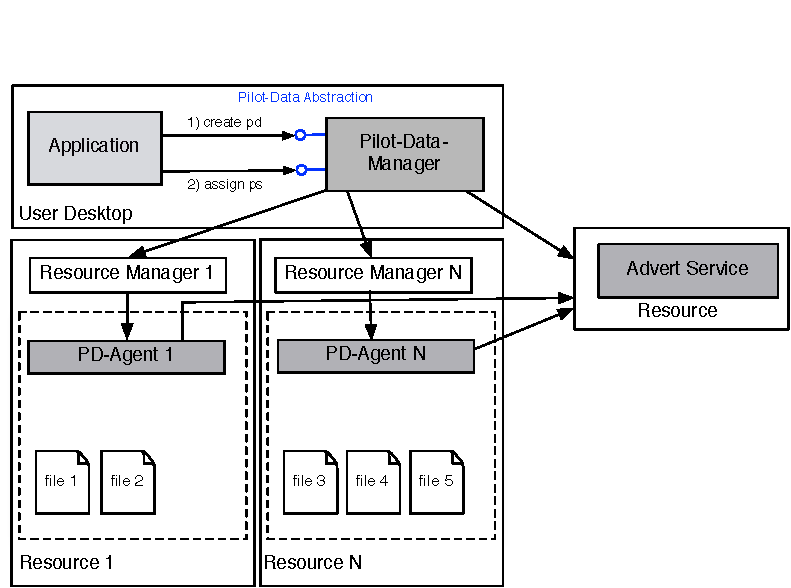
\includegraphics[width=\textwidth]{figures/pilot-data-manager.pdf}
%     \caption{\textbf{BigData Architecture:} The BD Manager exposes
%       TROY's PD API. Application can create group of files and assign 
%       files to storage. The BD manager tracks file locations in
%       the data catalog. The scheduler optimizes data-compute co-location.
%       The transfer manager initiates and monitors data movements. \up\up}
%     \label{fig:pilot-data-architecture}
%     \end{minipage}
% \end{figure*}

BigData-SAGA is the SAGA-based prototype of the Pilot-Data
abstraction; in the scope of this paper it is referred to as simply
BigData (BD).  Figure~\ref{fig:pilot-data-architecture} gives an
overview of the architecture.  The system consists of two components:
the BD manager, and the BD agents deployed on the physical
resources. The coordination scheme used is again M/W with some
intelligence that is located de-centrally at the BD agent. As
communication mechanism the SAGA Advert Service is used, in a similar
push/pull mode as for BJ.

The BD manager is responsible for 1) meta-data management, i.\,e.\ it
keeps track of the pilot stores that a pilot data object is associated
with, 2) for scheduling data movements and data replications (taking
into account the application requirements defined via affinities), and
3) for managing data movements activities.  Similar to BigJob, an
agent on each resource is used to manage the physical storage on a
resource.  

A particular critical requirement for data-intensive application, is
the management of affinity between DUs and also between WUs and
DUs. The BD scheduler supports preliminary affinity-aware
scheduling: both BigJob and BigData are tightly integrated to
efficiently support compute- and data-related aspects of dynamic
execution (see also \S{IIIA}).
 
\jhanote{Andre, please review the next paragraph: Should it just go
  for simplicity?} Thus, Pilot-Data introduces the PD container object
for expressing relationships between DUs. A PD corresponds to an SU in
the P* Model, i.\,e.\ it is used as scheduling unit for internal
optimizations, e.\,g.\ the grouping of DUs. Having instantiated a PD,
it can be assigned to a PS via the PD manager. A PS is a placeholder
reserving a certain amount of storage, i.\,e.\ it corresponds to a
pilot in the pilot-job model. By associating a PD to a PS the data is
actually moved to the physical location associated with the PS. The PD
manager facilitates the creation of PSs, schedules data movements
(with respect to specified affinities) and manages data accesses.


%%%%%%%%%%%%%%%%%%%%%%%%%%%%%%%%%%%%%%%%%%%%%%%%%%%%%%%%%%%%%%%%%%%%%%


% In addition to the three Pilot-Job framework discussed in this section, various
% other frameworks exist.
% \begin{itemize}
%     \item MyCluster~\cite{1652061} enables the 
% creation of a Condor, PBS or SGE clusters on-demand.
%     \item Falkon~\cite{1362680} is a Pilot-Job framework that emphasizes the 
% performance of its task dispatcher.
%     \item Nimrod/G~\cite{10.1109/HPC.2000.846563}
%     \item DIRAC~\cite{1742-6596-219-6-062049} is another pilot-job framework 
% used by the LHCb community.
%     \item ToPoS~\cite{topos} is a REST-based web service primarily designed with 
% respect to parameter sweep applications. Internally, ToPoS utilizes PJ 
% capabilities to efficiently manage resources.
%     \item The Production and Distributed Analysis System 
% (PanDA)~\cite{1742-6596-219-6-062041} is the workload management system of 
% the ATLAS experiment. PanDA utilizes multi-user PJs for resource management. 
% The PJ component is built on top of Condor-G and referred to as AutoPilot. 
% It can also be used independently of the ATLAS environment. 
% \end{itemize}



Both BigJob and BigData define similar elements that can be mapped to
each other. Nevertheless, compute and data model sometimes require a
different treatment.  The extended TROY (an implementation of the
extended P* Model) will optimize data- and computing according to a
set of defined affinities and policies.

% BJ and BD encapsulate cross-cutting properties across data and
% computation. 

% With the maturing of both models and
% implementations, we expect that both the PJ and PD model converge in
% the future.

\section{Discussion and Future Work \upp\upp}

% The P* model was used to demonstrate

The P* model provides a common framework for describing and
characterizing Pilot-abstractions. TROY is an implementation of the P*
model that captures the commonalities between the different PJ
implementations via a common API.  We validate the P* model by
demonstrating that the most widely used PJ frameworks, viz., DIANE,
Condor-G and SWIFT can be compared, contrasted and analyzed using this
framework, i.\,e.\ the architecture and the communication and
coordination schemes.

% We established PJ and PD as abstractions for supporting dynamic
% execution by decoupling workload and resource
% assignment/scheduling. 

% they share different important properties with respect to the commonly
% used communication and coordination schemes.

Having established the validity of the P* Model and TROY, in the
future, the TROY framework will be extended to support advanced
autonomic resource management and selection strategies, e.\,g.\ by
deploying more decentral decision logic into the agents. We will use
existing and emerging capabilities of TROY to support the efficient
and scalable solution of many scientific applications that involve
multiple independent tasks

% we will align the TROY API with the emerging SAGA Resource Management
% API~\cite{saga_rm}. We will further refine the TROY API, e.\,g.\ by
% generically supporting different security models via a context API
% (similar to the SAGA Context API).


%\note{work on scalability: Repex proposal?}

\up
\section*{Acknowledgements\upp\upp}
\footnotesize{This work is funded by Cybertools project
  (http://cybertools .loni.org; PI Jha) NSF/LEQSF
  (2007-10)-CyberRII-01, HPCOPS NSF-OCI 0710874 award, NSF-ExTENCI
  (OCI-1007115) and NIH Grant Number P20RR016456 from the NIH National
  Center For Research Resources. Important funding for SAGA has been
  provided by the UK EPSRC grant number GR/D0766171/1 (via OMII-UK).
  MS is sponsored by the program of BiG Grid, the Dutch e-Science
  Grid, which is financially supported by the Netherlands Organisation
  for Scientific Research, NWO. SJ acknowledges the e-Science
  Institute, Edinburgh for supporting the research
  theme. ``Distributed Programming Abstractions'' \& 3DPAS. We thank J
  Kim (CCT) for assistance with the DNA models.  SJ acknowledges
  useful related discussions with Jon Weissman (Minnesota) and Dan
  Katz (Chicago). This work has also been made possible thanks to
  computer resources provided by TeraGrid TRAC award TG-MCB090174
  (Jha). This document was developed with support from the National
  Science Foundation (NSF) under Grant No.  0910812 to Indiana
  University for ``FutureGrid: An Experimental, High-Performance Grid
  Test-bed.''.}

\up
\bibliographystyle{plain}
\bibliography{pilotjob,saga.bib,saga-related}
\end{document}


\note{Facilities provided include the creation of a PJ, insertion of
  tasks, and attachment to a CPU resource pool for late-binding task
  execution.}  \note{Tasks are ultimately loaded onto specific
  resources using the pilot-job and late-binding. In other words}
\note{PJ provides a mechanism to decouple “task coordination” from
  “resource mapping”.}
